\section{Artificial Bee Colony Algorithm}

The Artificial Bee Colony (ABC) algorithm is a nature-inspired, meta-heuristic optimisation
algorithm. It was introduced by Karaboga in \cite{beecolony}, and is motivated by the behaviour of honey bees.

The model defines three components: employed bees, unemployed bees, and food sources. Employed bees search for new food sources by searching in their neighbourhood. They show the gathered information to the unemployed bees, which get recruited by a probability dependent on the food source quality. Employed bees that where not able to improve the quality of their food source multiple times, will abandon this food source and become scout bees. Scouts are choosing their food source randomly.

Since we are seeking to solve the Travelling Salesman Problem (TSP), each food source is defined as a route of cities. Each city is defined by a x and a y coordinate. In the TSP we aim to get the optimal order of cities, which leads to a minimal travelling distance. We introduce problem specific knowledge to the algorithm by defining its neighbourhood search. Based on the idea from Li et al. \cite{beetsp}, we obtain the neighbour of a route by swapping the order of some cities. Each city will get swapped with a certain probability, and it will get swapped with a randomly chosen city.


\subsection{Experiments}

In this section we compare our implementation of the Artificial Bee Colony algorithm to the
reference evolutionary algorithm on the TSP problem.

As table \ref{tab:bee_vs_ea} and figure \ref{fig:bee_vs_ea} are showing, the ABC algorithm performed slightly worse than the reference evolutionary algorithm. As the standard deviations in table \ref{tab:bee_vs_ea} show, the results of the ABC algorithm where more stable when compared to the EA. 

For our tests we initialised 40 bees and optimise over 1000 iterations. We set the randomisation factor $\alpha = 0.005$, and the abandon-limit to 200.
The two approaches are very comparable in terms of their run-time, although the bee colony algorithm performs a higher number of evaluations over the same amount of iterations.

\begin{figure}[h]
	\centering
	\begin{subfigure}{.5\textwidth}
		\centering
		\captionsetup{width=0.75\linewidth}
		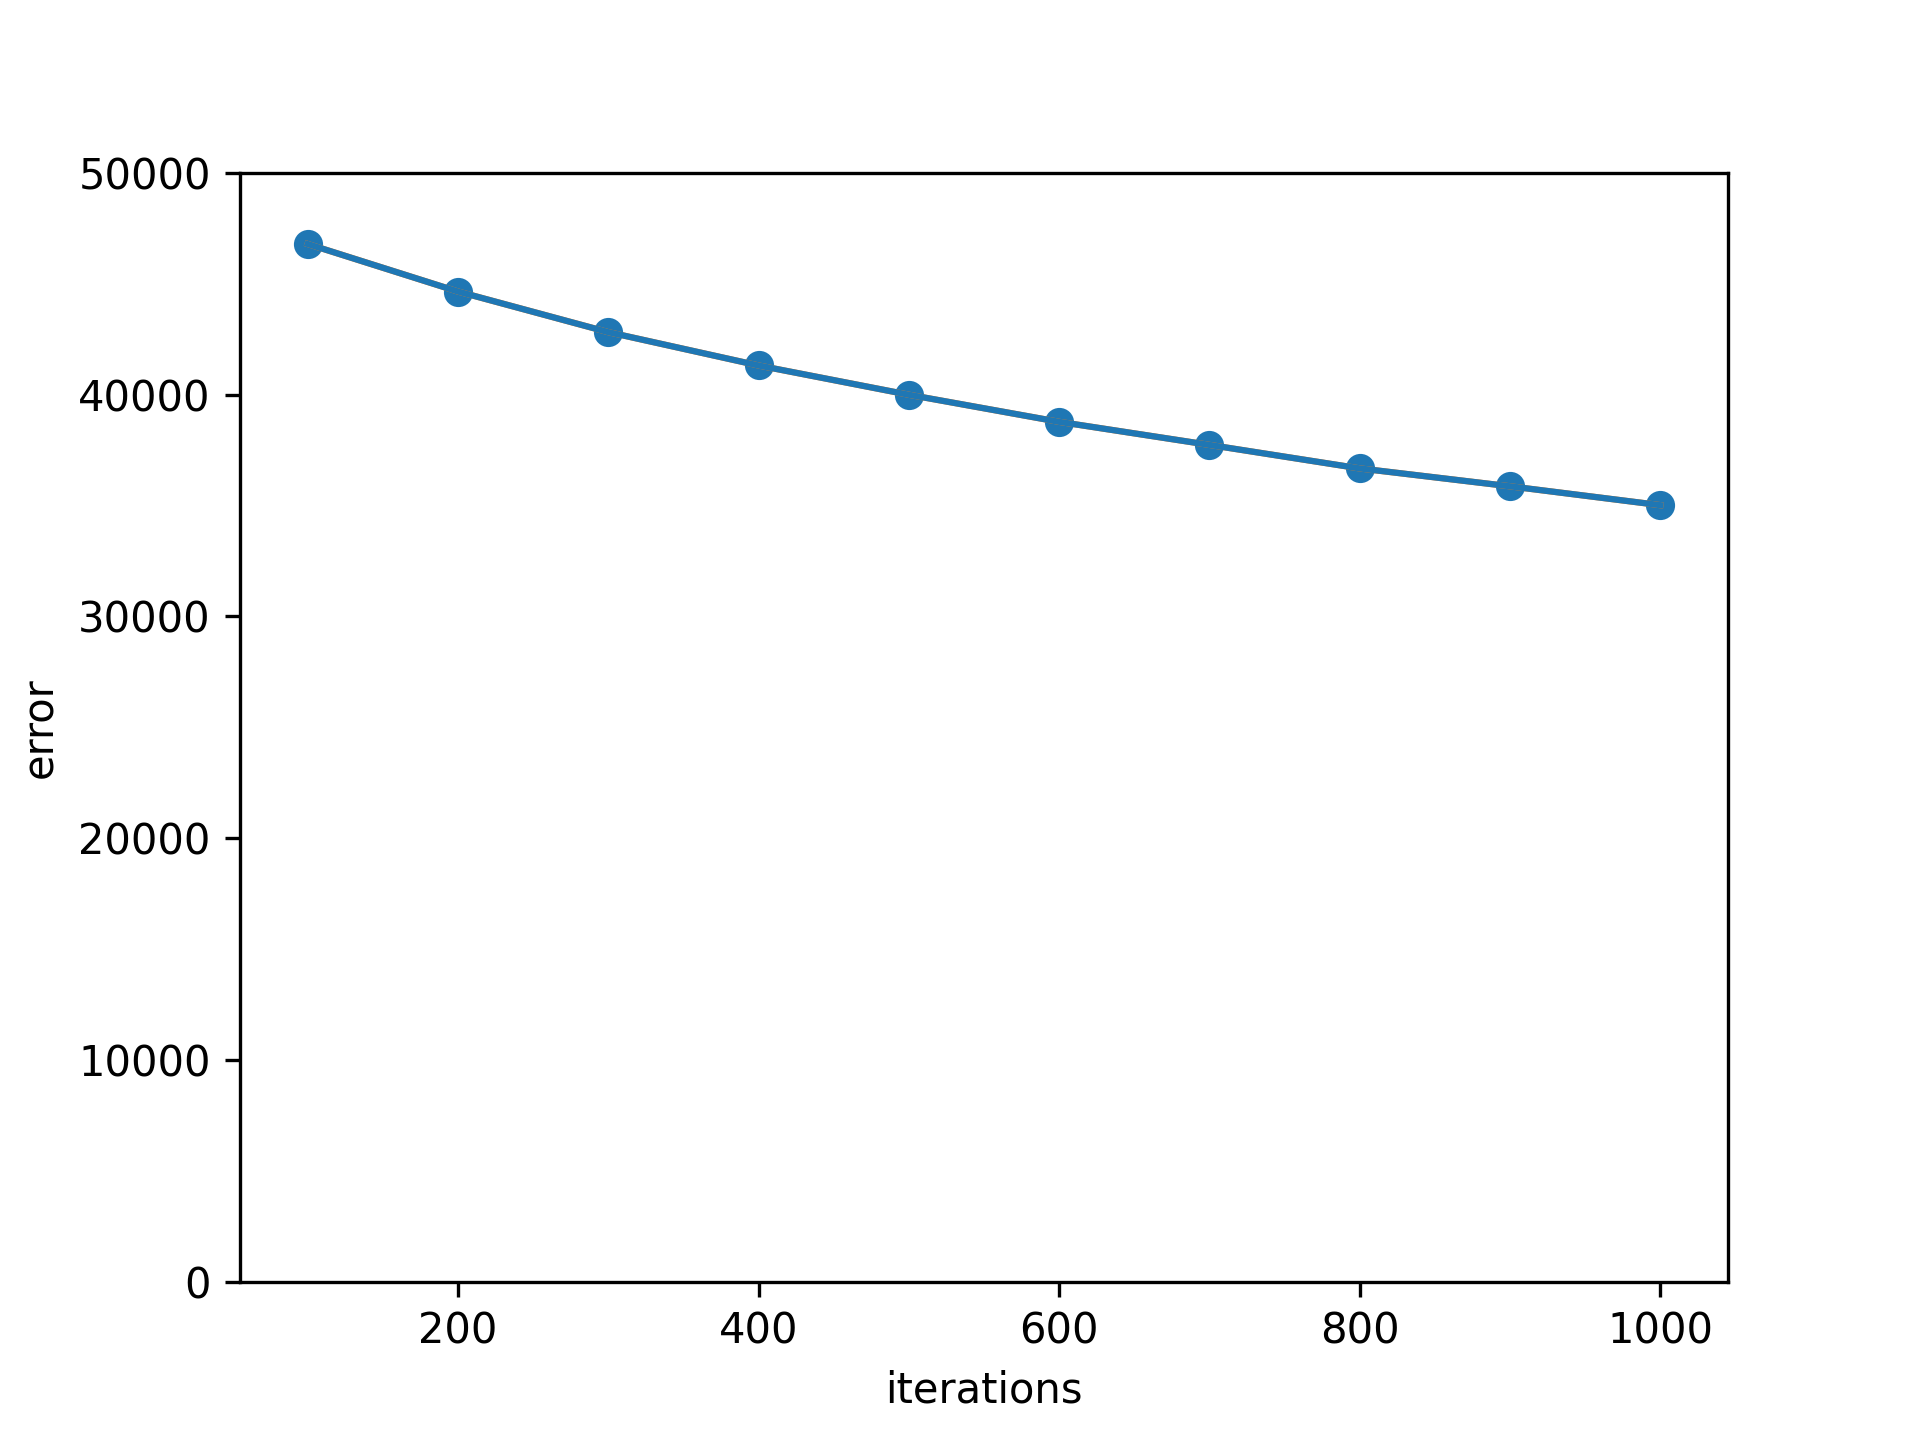
\includegraphics[width=0.75\linewidth]{assets/reference_tsp.png}
		\caption{Error over iterations using the reference evolutionary algorithm.}
		\label{fig:reference_tsp}
	\end{subfigure}%
	\begin{subfigure}{.5\textwidth}
		\centering
    \captionsetup{width=0.75\linewidth}
		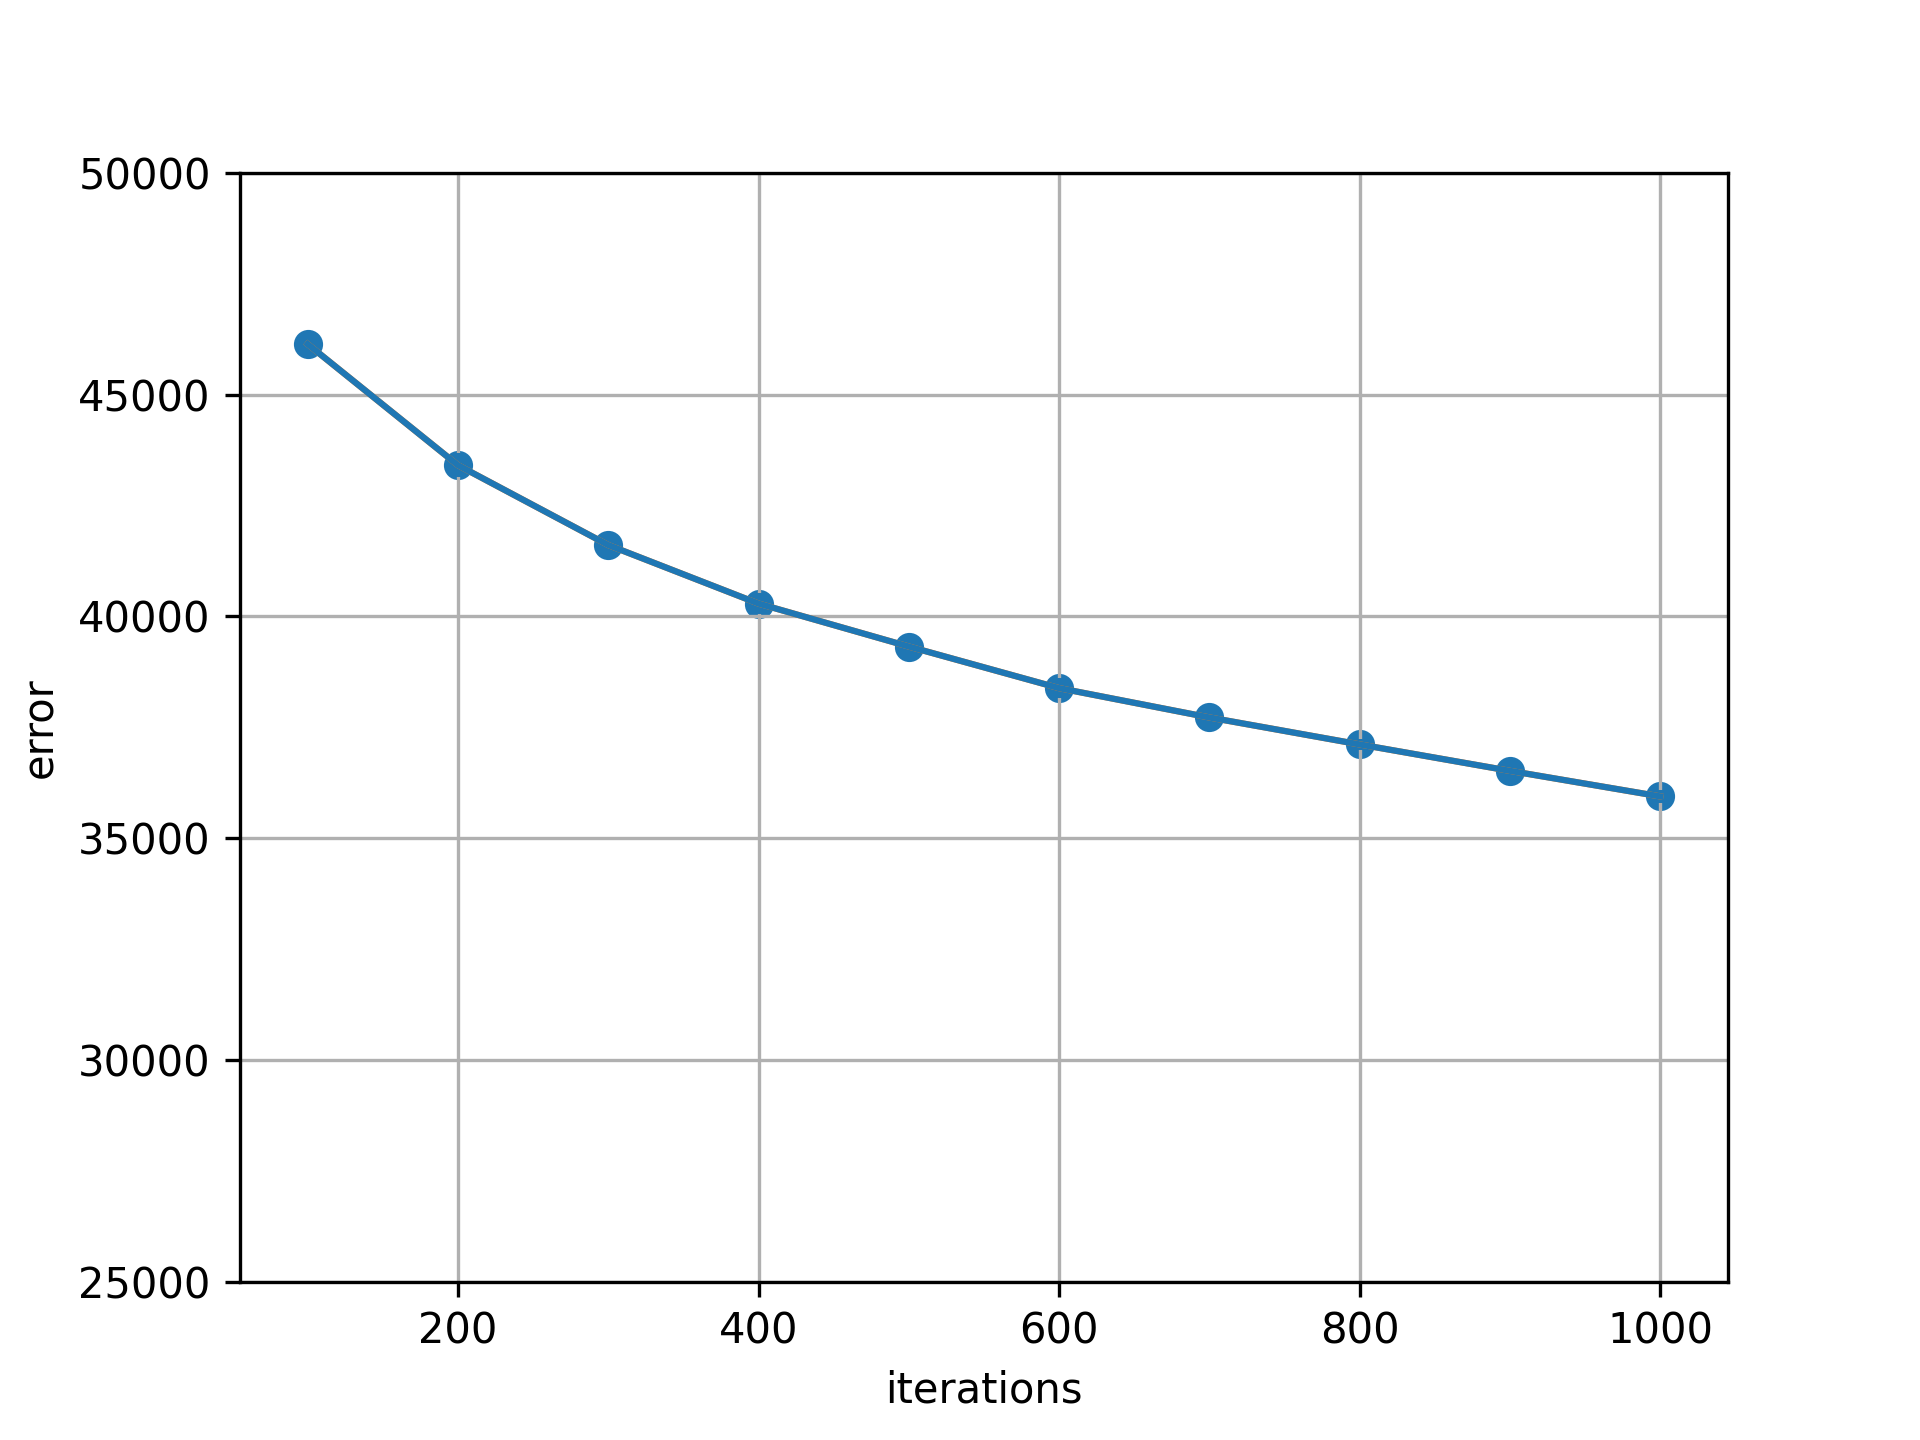
\includegraphics[width=0.75\linewidth]{assets/beecolony_tsp.png}
		\caption{Error over iterations using the bee colony algorithm.}
		\label{fig:becolony_tsp}
	\end{subfigure}
	\caption{Comparison of ABC and evolutionary algorithm on the TSP problem.}
	\label{fig:bee_vs_ea}
\end{figure}

\begin{table}[H]
	\centering
	\begin{tabular}{|c c c c|}
		\hline
		\textbf{Optimiser} & \textbf{Error} & \textbf{Evaluations} & \textbf{Run-time [s]} \\
		\hline
		Bee Colony Algorithm & $35939.18 \pm 144.21$ & 80040 & 2.93 \\
		Reference Evolutionary Algorithm & $35012.41 \pm 482.07$ & 25000 & 2.90 \\
		\hline
	\end{tabular}
	\caption{Minimal errors after the given number of evaluations produced by optimisers on the TSP problem. Results are averaged over 10 subsequent runs.}
	\label{tab:bee_vs_ea}
\end{table}
